% Options for packages loaded elsewhere
\PassOptionsToPackage{unicode}{hyperref}
\PassOptionsToPackage{hyphens}{url}
%
\documentclass[
]{article}
\usepackage{amsmath,amssymb}
\usepackage{lmodern}
\usepackage{ifxetex,ifluatex}
\ifnum 0\ifxetex 1\fi\ifluatex 1\fi=0 % if pdftex
  \usepackage[T1]{fontenc}
  \usepackage[utf8]{inputenc}
  \usepackage{textcomp} % provide euro and other symbols
\else % if luatex or xetex
  \usepackage{unicode-math}
  \defaultfontfeatures{Scale=MatchLowercase}
  \defaultfontfeatures[\rmfamily]{Ligatures=TeX,Scale=1}
\fi
% Use upquote if available, for straight quotes in verbatim environments
\IfFileExists{upquote.sty}{\usepackage{upquote}}{}
\IfFileExists{microtype.sty}{% use microtype if available
  \usepackage[]{microtype}
  \UseMicrotypeSet[protrusion]{basicmath} % disable protrusion for tt fonts
}{}
\makeatletter
\@ifundefined{KOMAClassName}{% if non-KOMA class
  \IfFileExists{parskip.sty}{%
    \usepackage{parskip}
  }{% else
    \setlength{\parindent}{0pt}
    \setlength{\parskip}{6pt plus 2pt minus 1pt}}
}{% if KOMA class
  \KOMAoptions{parskip=half}}
\makeatother
\usepackage{xcolor}
\IfFileExists{xurl.sty}{\usepackage{xurl}}{} % add URL line breaks if available
\IfFileExists{bookmark.sty}{\usepackage{bookmark}}{\usepackage{hyperref}}
\hypersetup{
  hidelinks,
  pdfcreator={LaTeX via pandoc}}
\urlstyle{same} % disable monospaced font for URLs
\usepackage[margin=1in]{geometry}
\usepackage{color}
\usepackage{fancyvrb}
\newcommand{\VerbBar}{|}
\newcommand{\VERB}{\Verb[commandchars=\\\{\}]}
\DefineVerbatimEnvironment{Highlighting}{Verbatim}{commandchars=\\\{\}}
% Add ',fontsize=\small' for more characters per line
\usepackage{framed}
\definecolor{shadecolor}{RGB}{248,248,248}
\newenvironment{Shaded}{\begin{snugshade}}{\end{snugshade}}
\newcommand{\AlertTok}[1]{\textcolor[rgb]{0.94,0.16,0.16}{#1}}
\newcommand{\AnnotationTok}[1]{\textcolor[rgb]{0.56,0.35,0.01}{\textbf{\textit{#1}}}}
\newcommand{\AttributeTok}[1]{\textcolor[rgb]{0.77,0.63,0.00}{#1}}
\newcommand{\BaseNTok}[1]{\textcolor[rgb]{0.00,0.00,0.81}{#1}}
\newcommand{\BuiltInTok}[1]{#1}
\newcommand{\CharTok}[1]{\textcolor[rgb]{0.31,0.60,0.02}{#1}}
\newcommand{\CommentTok}[1]{\textcolor[rgb]{0.56,0.35,0.01}{\textit{#1}}}
\newcommand{\CommentVarTok}[1]{\textcolor[rgb]{0.56,0.35,0.01}{\textbf{\textit{#1}}}}
\newcommand{\ConstantTok}[1]{\textcolor[rgb]{0.00,0.00,0.00}{#1}}
\newcommand{\ControlFlowTok}[1]{\textcolor[rgb]{0.13,0.29,0.53}{\textbf{#1}}}
\newcommand{\DataTypeTok}[1]{\textcolor[rgb]{0.13,0.29,0.53}{#1}}
\newcommand{\DecValTok}[1]{\textcolor[rgb]{0.00,0.00,0.81}{#1}}
\newcommand{\DocumentationTok}[1]{\textcolor[rgb]{0.56,0.35,0.01}{\textbf{\textit{#1}}}}
\newcommand{\ErrorTok}[1]{\textcolor[rgb]{0.64,0.00,0.00}{\textbf{#1}}}
\newcommand{\ExtensionTok}[1]{#1}
\newcommand{\FloatTok}[1]{\textcolor[rgb]{0.00,0.00,0.81}{#1}}
\newcommand{\FunctionTok}[1]{\textcolor[rgb]{0.00,0.00,0.00}{#1}}
\newcommand{\ImportTok}[1]{#1}
\newcommand{\InformationTok}[1]{\textcolor[rgb]{0.56,0.35,0.01}{\textbf{\textit{#1}}}}
\newcommand{\KeywordTok}[1]{\textcolor[rgb]{0.13,0.29,0.53}{\textbf{#1}}}
\newcommand{\NormalTok}[1]{#1}
\newcommand{\OperatorTok}[1]{\textcolor[rgb]{0.81,0.36,0.00}{\textbf{#1}}}
\newcommand{\OtherTok}[1]{\textcolor[rgb]{0.56,0.35,0.01}{#1}}
\newcommand{\PreprocessorTok}[1]{\textcolor[rgb]{0.56,0.35,0.01}{\textit{#1}}}
\newcommand{\RegionMarkerTok}[1]{#1}
\newcommand{\SpecialCharTok}[1]{\textcolor[rgb]{0.00,0.00,0.00}{#1}}
\newcommand{\SpecialStringTok}[1]{\textcolor[rgb]{0.31,0.60,0.02}{#1}}
\newcommand{\StringTok}[1]{\textcolor[rgb]{0.31,0.60,0.02}{#1}}
\newcommand{\VariableTok}[1]{\textcolor[rgb]{0.00,0.00,0.00}{#1}}
\newcommand{\VerbatimStringTok}[1]{\textcolor[rgb]{0.31,0.60,0.02}{#1}}
\newcommand{\WarningTok}[1]{\textcolor[rgb]{0.56,0.35,0.01}{\textbf{\textit{#1}}}}
\usepackage{graphicx}
\makeatletter
\def\maxwidth{\ifdim\Gin@nat@width>\linewidth\linewidth\else\Gin@nat@width\fi}
\def\maxheight{\ifdim\Gin@nat@height>\textheight\textheight\else\Gin@nat@height\fi}
\makeatother
% Scale images if necessary, so that they will not overflow the page
% margins by default, and it is still possible to overwrite the defaults
% using explicit options in \includegraphics[width, height, ...]{}
\setkeys{Gin}{width=\maxwidth,height=\maxheight,keepaspectratio}
% Set default figure placement to htbp
\makeatletter
\def\fps@figure{htbp}
\makeatother
\setlength{\emergencystretch}{3em} % prevent overfull lines
\providecommand{\tightlist}{%
  \setlength{\itemsep}{0pt}\setlength{\parskip}{0pt}}
\setcounter{secnumdepth}{-\maxdimen} % remove section numbering
\ifluatex
  \usepackage{selnolig}  % disable illegal ligatures
\fi
\newlength{\cslhangindent}
\setlength{\cslhangindent}{1.5em}
\newlength{\csllabelwidth}
\setlength{\csllabelwidth}{3em}
\newenvironment{CSLReferences}[2] % #1 hanging-ident, #2 entry spacing
 {% don't indent paragraphs
  \setlength{\parindent}{0pt}
  % turn on hanging indent if param 1 is 1
  \ifodd #1 \everypar{\setlength{\hangindent}{\cslhangindent}}\ignorespaces\fi
  % set entry spacing
  \ifnum #2 > 0
  \setlength{\parskip}{#2\baselineskip}
  \fi
 }%
 {}
\usepackage{calc}
\newcommand{\CSLBlock}[1]{#1\hfill\break}
\newcommand{\CSLLeftMargin}[1]{\parbox[t]{\csllabelwidth}{#1}}
\newcommand{\CSLRightInline}[1]{\parbox[t]{\linewidth - \csllabelwidth}{#1}\break}
\newcommand{\CSLIndent}[1]{\hspace{\cslhangindent}#1}

\author{}
\date{\vspace{-2.5em}}

\begin{document}

\begin{center}\rule{0.5\linewidth}{0.5pt}\end{center}

Self Organizing Maps

R Programming, FOSSEE Team

\begin{center}\rule{0.5\linewidth}{0.5pt}\end{center}

\hypertarget{table-of-contents}{%
\section{Table of Contents}\label{table-of-contents}}

\begin{itemize}
\tightlist
\item
  Chapter 1: Introduction to SOM
\item
  Chapter 2: Algorithm
\item
  Chapter 3: Guided Tutorial in R -- 3.1: Initialization -- 3.2:
  Sampling -- 3.3: Competition -- 3.4: Cooperation -- 3.5: Adaptation
\item
  Chapter 4: Implementation -- 4.1: Data Generation -- 4.2:
  Initialization -- 4.3: Best Matching Unit -- 4.4:Training the SOM
\item
  Chapter 5: Optimization in R
\item
  Chapter 6: References
\end{itemize}

\hypertarget{chapter-1-introduction-to-som}{%
\subsection{Chapter 1: Introduction to
SOM}\label{chapter-1-introduction-to-som}}

Self organizing maps are a class of artificial neural networks based on
competitive learning that helps to organize and understand high
dimensional data by reducing the number of dimensions from a high
dimensional space to a 2 D map. With SOM, clustering is performed by
having several units compete for the current object. Once the data have
been entered into the system, the newtwork of artificial neurons is
trained by providing information about inputs. The weight vector of the
unit is closest to the current object becomes the winning or active
unit. During the training stage, the values for the input variables are
gradually adjusted in an attempt to preserve neighborhood relationships
that exist within the input data set. As it gets closer to the input
object, the weights of the winning unit are adjusted as well as its
neighbors.(Uoolc, n.d.)

\begin{figure}
\centering
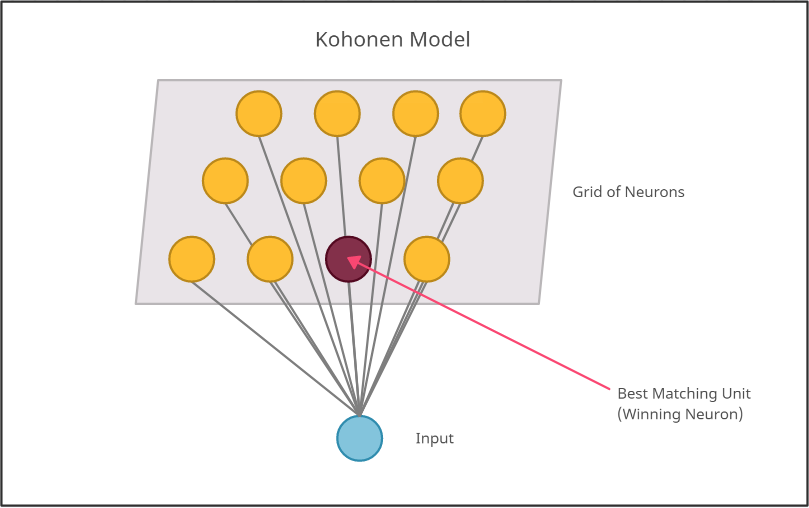
\includegraphics{model.png}
\caption{Figure 1: Kohonen model}
\end{figure}

\hypertarget{competitive-learning}{%
\paragraph{Competitive Learning}\label{competitive-learning}}

The model utilizes using unsupervised learning to map the input through
competitive learning in which the output neurons compete amongst
themselves to be activated, with the result that only one is activated
at any one time. Getting the Best Matching Unit is done by running
through all wright vectors and calculating the distance from each weight
to the sample vector. The weight with the shortest distance is the
winner. There are numerous ways to determine the distance, however, the
most commonly used method is the Euclidean Distance and/or Consine
Distance.Due to the negative feedback connections between the neurons,
the neurons are forced to organise themselves which gave rise to the
name Self Organizing Map (SOM).

\begin{figure}
\centering
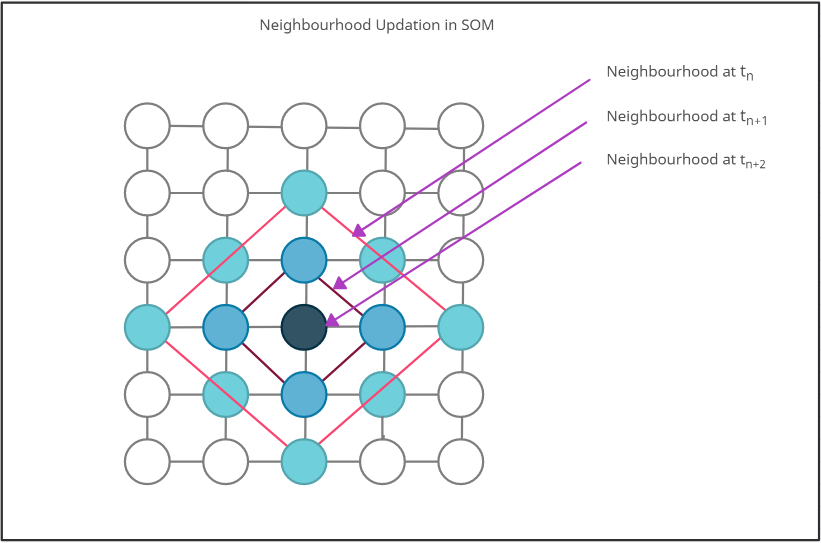
\includegraphics{neigh.png}
\caption{Figure 2: Updating neighbourhood after finding BMU}
\end{figure}

\hypertarget{chapter-2-algorithm}{%
\subsection{Chapter 2: Algorithm}\label{chapter-2-algorithm}}

\begin{figure}
\centering
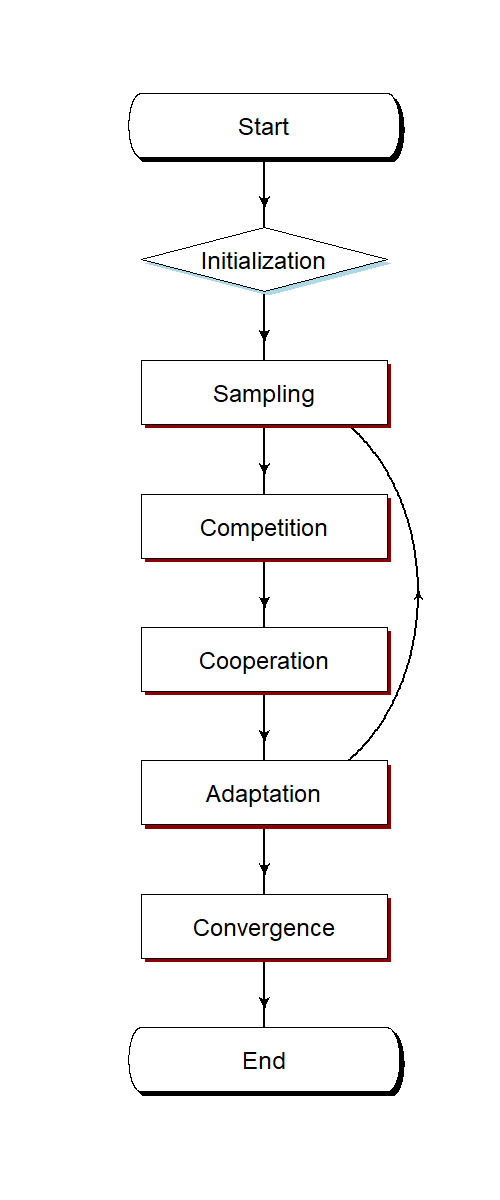
\includegraphics{flowchart.png}
\caption{Figure 3: Flowchart}
\end{figure}

\hypertarget{steps}{%
\subsubsection{Steps:}\label{steps}}

\begin{itemize}
\tightlist
\item
  Initialization - Create a grid of neurons and randomly initialize
  weights.
\item
  Sampling- Select a random row (vector) from input data.
\item
  Competition- Neurons fight to become the Best Matching Unit which is
  determined using the discriminant function.
\item
  Cooperation- The winning neuron determines the spatial location of a
  topological neighbourhood of excited neurons which will cooperate.
\item
  Adaptation- Weights are adjusted with respect to winning neuron, such
  that a similar input pattern is enhanced.
\item
  We will go back to step 2 and keep repeating the process till the map
  stops changing or convergence is achieved.
\end{itemize}

\hypertarget{chapter-3-guided-tutorial-in-r}{%
\subsection{Chapter 3: Guided Tutorial in
R}\label{chapter-3-guided-tutorial-in-r}}

\hypertarget{initialization}{%
\subsubsection{3.1: Initialization}\label{initialization}}

Create a grid of neurons and randomly initialize weights. The neurons
are represented by weight vectors of same dimensions as input. The
random numbers are generated using the rnorm function which generates
random numbers in the range -1 to 1.

Code snippet:

\begin{Shaded}
\begin{Highlighting}[]
\CommentTok{\#Let\textquotesingle{}s create a matrix of 10 rows and 5 columns}
\NormalTok{t }\OtherTok{\textless{}{-}} \FunctionTok{matrix}\NormalTok{(}\AttributeTok{data =} \FunctionTok{rnorm}\NormalTok{(}\DecValTok{50}\NormalTok{),  }\AttributeTok{nrow =}\NormalTok{ (}\DecValTok{10}\NormalTok{), }\AttributeTok{ncol =} \DecValTok{5}\NormalTok{)}
\NormalTok{t}
\end{Highlighting}
\end{Shaded}

\begin{verbatim}
##              [,1]       [,2]        [,3]       [,4]        [,5]
##  [1,] -0.30572921  0.3016526  0.71568932 -0.9730824 -0.50138860
##  [2,]  0.53953523 -1.0329605  0.75544328  0.1089760  0.23326648
##  [3,]  0.02294188  0.7235556  0.01487201 -1.7995189 -2.49854327
##  [4,]  1.00803848 -1.9833099  1.22280668 -0.5415011  1.20535529
##  [5,]  0.85162083  0.4498542 -0.32960184  0.2300291  0.60426298
##  [6,]  2.33843709 -0.7742256 -0.58378928  0.1051464 -0.14630167
##  [7,]  0.50694563 -0.4773714  0.29271876  0.5955806 -0.08675895
##  [8,]  3.22952931  0.9190880 -0.70202607 -0.3398997 -1.19167110
##  [9,]  0.82097794  1.0554806 -0.94971231 -3.2821712 -1.72553142
## [10,]  0.41790940 -0.7447319 -0.03896350  0.6340060  0.30499733
\end{verbatim}

\hypertarget{sampling}{%
\subsubsection{3.2: Sampling}\label{sampling}}

Select a random row (vector) from input data. The sampling is done using
the sample() function in R which retrieves an input row.

\begin{Shaded}
\begin{Highlighting}[]
\NormalTok{i }\OtherTok{\textless{}{-}} \FunctionTok{sample}\NormalTok{(t, }\DecValTok{1}\NormalTok{, }\AttributeTok{replace =}\NormalTok{ F)}
\NormalTok{i}
\end{Highlighting}
\end{Shaded}

\begin{verbatim}
## [1] 0.4498542
\end{verbatim}

\hypertarget{competition}{%
\subsubsection{3.3: Competition}\label{competition}}

Neurons fight to become the Best Matching Unit which is determined using
the discriminant function.Here our discriminant function is Euclidean
distance given by the formula:

\begin{equation}
 d\left( x,y\right) = \sqrt {\sum _{i=1}^{n}  \left( y_{i}- x_{i}\right)^2 } 
 \end{equation} where \(x\) and \(y\) are the two points in n
dimensional space and \(x_{i}\) and \(y_{i}\) are the vectors
representing their positions between which the Euclidean distance is to
be calculated.

Euclidean distance formula

\begin{Shaded}
\begin{Highlighting}[]
\CommentTok{\#Lets make a function to calculate euclidean distance.}
\NormalTok{euclidean\_distance }\OtherTok{\textless{}{-}} \ControlFlowTok{function}\NormalTok{(x, y) \{}
\NormalTok{  ret }\OtherTok{\textless{}{-}} \FunctionTok{sum}\NormalTok{((x }\SpecialCharTok{{-}}\NormalTok{ y)}\SpecialCharTok{\^{}}\DecValTok{2}\NormalTok{)}
  \FunctionTok{return}\NormalTok{(ret)}
\NormalTok{\}}

\CommentTok{\#Let\textquotesingle{}s run this on a sample input}

\FunctionTok{euclidean\_distance}\NormalTok{(}\DecValTok{2}\NormalTok{,}\DecValTok{4}\NormalTok{)}
\end{Highlighting}
\end{Shaded}

\begin{verbatim}
## [1] 4
\end{verbatim}

The Best Matching Unit is the neuron which is closest to the input
vector. The discriminant function is used to calculate this distance
between all the neurons' weights and the input vector.

\begin{figure}
\centering
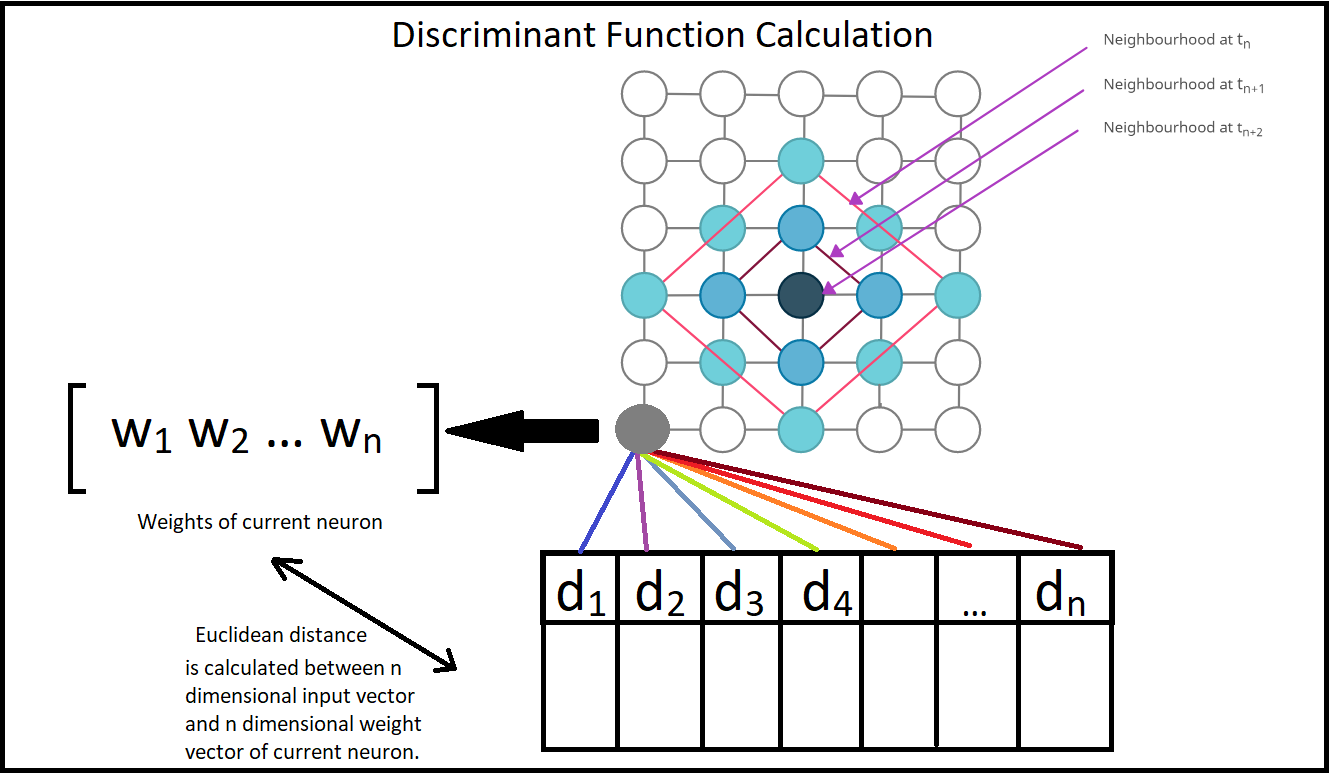
\includegraphics{dis.png}
\caption{Figure 4: Discriminant function calculation}
\end{figure}

\begin{Shaded}
\begin{Highlighting}[]
\CommentTok{\# x is a single input row of data and input\_grid is the grid}
\NormalTok{BMU }\OtherTok{\textless{}{-}} \ControlFlowTok{function}\NormalTok{(x, input\_grid) \{ }
\NormalTok{  distance }\OtherTok{\textless{}{-}} \DecValTok{0}
\NormalTok{  min\_distance }\OtherTok{\textless{}{-}} \DecValTok{10000000} \CommentTok{\# Setting high min dist value}
\NormalTok{  min\_ind }\OtherTok{\textless{}{-}} \SpecialCharTok{{-}}\DecValTok{1} \CommentTok{\# Setting random min\_ind value}
  \ControlFlowTok{for}\NormalTok{ (e }\ControlFlowTok{in} \DecValTok{1}\SpecialCharTok{:}\FunctionTok{nrow}\NormalTok{(input\_grid)) }\CommentTok{\# Iterating through grid}
\NormalTok{  \{}
\NormalTok{    distance }\OtherTok{\textless{}{-}} \FunctionTok{euclidean\_distance}\NormalTok{(x, input\_grid[e, ]) }\CommentTok{\# euclidean\_distance distance}
    \ControlFlowTok{if}\NormalTok{ (distance }\SpecialCharTok{\textless{}}\NormalTok{ min\_distance) \{}
\NormalTok{      min\_distance }\OtherTok{\textless{}{-}}\NormalTok{ distance }\CommentTok{\# Updating min distance for winning unit}
\NormalTok{      min\_ind }\OtherTok{\textless{}{-}}\NormalTok{ e }\CommentTok{\# Updating winning neuron}
\NormalTok{    \}}
\NormalTok{  \}}
  \FunctionTok{return}\NormalTok{(min\_ind}\DecValTok{{-}1}\NormalTok{) }\CommentTok{\#returns index of BMU}
\NormalTok{\}}
\end{Highlighting}
\end{Shaded}

\hypertarget{cooperation}{%
\subsubsection{3.4: Cooperation}\label{cooperation}}

The winning neuron determines the spatial location of a topological
neighbourhood of excited neurons which will cooperate.

\begin{equation}
 influence = exp(-(distance^{2}) / (2 * (radius^{2}))) 
 \end{equation} where \(distance\) is the lateral distance between
neurons in the grid and \(radius\) is the radius of the neighbourhood
over which influence is to be calculated.

Neighbourhood influence calculation formula

\begin{Shaded}
\begin{Highlighting}[]
\CommentTok{\# Defining a function to calculate the neighbourhood influence using the radius of neighbourhood and lateral distance.}
\NormalTok{influence\_calculation }\OtherTok{\textless{}{-}} \ControlFlowTok{function}\NormalTok{(distance, radius) \{}
\NormalTok{  ret }\OtherTok{\textless{}{-}} \FunctionTok{exp}\NormalTok{(}\SpecialCharTok{{-}}\NormalTok{(distance}\SpecialCharTok{\^{}}\DecValTok{2}\NormalTok{) }\SpecialCharTok{/}\NormalTok{ (}\DecValTok{2} \SpecialCharTok{*}\NormalTok{ (radius}\SpecialCharTok{\^{}}\DecValTok{2}\NormalTok{)))}
  \FunctionTok{return}\NormalTok{(ret)}
\NormalTok{\}}

\CommentTok{\# Calculating sample neighbourhood for lateral distance 2 and radius 4.}
\FunctionTok{influence\_calculation}\NormalTok{(}\DecValTok{2}\NormalTok{,}\DecValTok{4}\NormalTok{)}
\end{Highlighting}
\end{Shaded}

\begin{verbatim}
## [1] 0.8824969
\end{verbatim}

\hypertarget{adaptation}{%
\subsubsection{3.5: Adaptation}\label{adaptation}}

Weights are adjusted with respect to winning neuron, such that a similar
input pattern is enhanced.

\begin{equation}
 new\_radius = radius * exp(-current\_iteration / time\_constant) 
 \end{equation} where \(radius\) is the initial radius of neighbourhood,
\(current\_iteration\) is the iteration of data sampling that we are
currently on and \(time\_constant\) is the time constant which is
incremented at each iteration, when the SOM gets updated.

Radius decay formula

\textless{}\body\textgreater{}

\begin{Shaded}
\begin{Highlighting}[]
\CommentTok{\#Function for the decaying radius for a given iteration current\_iteration}
\NormalTok{decay\_radius\_function }\OtherTok{\textless{}{-}} \ControlFlowTok{function}\NormalTok{(radius, current\_iteration, time\_constant) \{}
\NormalTok{  ret }\OtherTok{\textless{}{-}}\NormalTok{ radius }\SpecialCharTok{*} \FunctionTok{exp}\NormalTok{(}\SpecialCharTok{{-}}\NormalTok{current\_iteration }\SpecialCharTok{/}\NormalTok{ time\_constant)}
  \FunctionTok{return}\NormalTok{(ret)}
\NormalTok{\}}

\CommentTok{\# Calculate radius of neighborhood at a iteration 4, with radius 3 and at the 4th iteration}
\FunctionTok{decay\_radius\_function}\NormalTok{(}\DecValTok{3}\NormalTok{,}\DecValTok{4}\NormalTok{,}\DecValTok{4}\NormalTok{)}
\end{Highlighting}
\end{Shaded}

\begin{verbatim}
## [1] 1.103638
\end{verbatim}

\begin{equation}
 new\_lateral\_distance = learning\_rate * exp(-current\_iteration / n\_iteration)
 \end{equation} where \(learning\_rate\) is the old learning rate to be
updated, \(current\_iteration\) is the iteration of data sampling that
we are currently on and \(n\_iteration\) is the total number of
iterations the SOM is trained over.

Learning rate decay formula

\begin{Shaded}
\begin{Highlighting}[]
\CommentTok{\#Function for the decaying learning rate}
\NormalTok{decay\_learning\_rate }\OtherTok{\textless{}{-}} \ControlFlowTok{function}\NormalTok{(learning\_rate, current\_iteration, n\_iteration) \{}
\NormalTok{  ret }\OtherTok{\textless{}{-}}\NormalTok{ learning\_rate }\SpecialCharTok{*} \FunctionTok{exp}\NormalTok{(}\SpecialCharTok{{-}}\NormalTok{current\_iteration }\SpecialCharTok{/}\NormalTok{ n\_iteration)}
  \FunctionTok{return}\NormalTok{(ret)}
\NormalTok{\}}

\CommentTok{\#Calculating the learning rate of model at the 3rd iteration out of a total of 100 iterations and initial learning rate of 0.1.}
\FunctionTok{decay\_learning\_rate}\NormalTok{(}\FloatTok{0.1}\NormalTok{,}\DecValTok{3}\NormalTok{,}\DecValTok{100}\NormalTok{)}
\end{Highlighting}
\end{Shaded}

\begin{verbatim}
## [1] 0.09704455
\end{verbatim}

\hypertarget{chapter-4-implementation}{%
\subsection{Chapter 4: Implementation}\label{chapter-4-implementation}}

\hypertarget{data-generation}{%
\subsubsection{4.1: Data Generation}\label{data-generation}}

For this tutorial, we will demonstrate the working of SOM on a given
dataset of 3 dimensions. We will load this dataset from the working
directory. We will also import the necessary libraries.

Code Snippet

\begin{Shaded}
\begin{Highlighting}[]
\FunctionTok{set.seed}\NormalTok{(}\DecValTok{222}\NormalTok{)}
\FunctionTok{library}\NormalTok{(dplyr)}

\CommentTok{\# 1) Reading the data and scaling it}
\NormalTok{data }\OtherTok{\textless{}{-}} \FunctionTok{read.csv}\NormalTok{(}\StringTok{"binary.csv"}\NormalTok{, }\AttributeTok{header =}\NormalTok{ T)}
\NormalTok{X }\OtherTok{\textless{}{-}} \FunctionTok{scale}\NormalTok{(data[, }\SpecialCharTok{{-}}\DecValTok{1}\NormalTok{])}
\NormalTok{data }\OtherTok{\textless{}{-}}\NormalTok{ X}
\end{Highlighting}
\end{Shaded}

\hypertarget{initialization-1}{%
\subsubsection{4.2: Initialization}\label{initialization-1}}

The SOM is in its essence a grid of neurons, each neuron containing a
weight vector and a position i,j in the grid. We begin by assigning
random values for the initial weight vectors w. The dimensions of the
weight vector are equal to the number of input dimensions.

\begin{figure}
\centering
\includegraphics{W.png}
\caption{Figure 5: Weights matrix}
\end{figure}

Code Snippet

\begin{Shaded}
\begin{Highlighting}[]
\CommentTok{\#Now lets initialize the weights of the neural network.}
\CommentTok{\#Creating a 4x4 neural network with 3 dimensions to match the input.}

\CommentTok{\# {-}{-}{-}{-}{-}{-}{-}{-}{-}{-}{-}{-}{-}{-}{-}{-}{-}{-}{-}{-}{-}{-}{-}{-}{-}{-}{-}{-}{-}{-}{-}{-}{-}{-}{-}{-}{-}{-}{-}{-}{-}{-}{-}{-}{-}{-}{-}{-}{-}{-}{-}{-}{-}}
\CommentTok{\# This is Step 1 of the Algorithm: Initialization}
\CommentTok{\# {-}{-}{-}{-}{-}{-}{-}{-}{-}{-}{-}{-}{-}{-}{-}{-}{-}{-}{-}{-}{-}{-}{-}{-}{-}{-}{-}{-}{-}{-}{-}{-}{-}{-}{-}{-}{-}{-}{-}{-}{-}{-}{-}{-}{-}{-}{-}{-}{-}{-}{-}{-}{-}}

\NormalTok{create\_grid }\OtherTok{\textless{}{-}} \ControlFlowTok{function}\NormalTok{(n,p) \{}
\NormalTok{  ret }\OtherTok{\textless{}{-}} \FunctionTok{matrix}\NormalTok{(}\AttributeTok{data =} \FunctionTok{rnorm}\NormalTok{(n }\SpecialCharTok{*}\NormalTok{ p), }\AttributeTok{nrow =}\NormalTok{ n, }\AttributeTok{ncol =}\NormalTok{ p)}
  \FunctionTok{return}\NormalTok{(ret)}
\NormalTok{\}}
\NormalTok{grid }\OtherTok{\textless{}{-}} \FunctionTok{create\_grid}\NormalTok{(}\DecValTok{16}\NormalTok{,}\DecValTok{3}\NormalTok{)}
\NormalTok{grid}
\end{Highlighting}
\end{Shaded}

\begin{verbatim}
##               [,1]         [,2]       [,3]
##  [1,]  1.487757090 -2.005512989 -0.2154811
##  [2,] -0.001891901  0.007509885 -0.1146497
##  [3,]  1.381020790  0.519490356 -0.2022654
##  [4,] -0.380213631 -0.746295471  0.4064927
##  [5,]  0.184136230  0.726454576  0.6567724
##  [6,] -0.246895883  0.713656667  0.1061908
##  [7,] -1.215560910 -0.650062920 -0.1843974
##  [8,]  1.561405098  1.498696215  0.9460342
##  [9,]  0.427310197 -1.435828082  0.2023869
## [10,] -1.201023506 -2.161318185  0.4951010
## [11,]  1.052458495  0.395219851 -0.5693554
## [12,] -1.305063566 -0.394833956  1.1192945
## [13,] -0.692607634 -0.309758382  2.2090779
## [14,]  0.602648854  1.330826619  0.3171826
## [15,] -0.197753074 -0.817428629 -0.9352971
## [16,] -1.185874517  0.675893491  0.8136619
\end{verbatim}

\#\#\# 4.3: Best Matching Unit

The SOM works using competitive learning which selects a best matching
unit at each iteration using the discriminant function value closest to
the randomly sampled input vector.

Code Snippet

\begin{Shaded}
\begin{Highlighting}[]
\CommentTok{\# {-}{-}{-}{-}{-}{-}{-}{-}{-}{-}{-}{-}{-}{-}{-}{-}{-}{-}{-}{-}{-}{-}{-}{-}{-}{-}{-}{-}{-}{-}{-}{-}{-}{-}{-}{-}{-}{-}{-}{-}{-}{-}{-}{-}{-}{-}{-}{-}{-}{-}{-}{-}{-}}
\CommentTok{\# This is Step 3 of the Algorithm: Competition}
\CommentTok{\# {-}{-}{-}{-}{-}{-}{-}{-}{-}{-}{-}{-}{-}{-}{-}{-}{-}{-}{-}{-}{-}{-}{-}{-}{-}{-}{-}{-}{-}{-}{-}{-}{-}{-}{-}{-}{-}{-}{-}{-}{-}{-}{-}{-}{-}{-}{-}{-}{-}{-}{-}{-}{-}}

\CommentTok{\# euclidean\_distance function}
\NormalTok{euclidean\_distance }\OtherTok{\textless{}{-}} \ControlFlowTok{function}\NormalTok{(x, y) \{}
\NormalTok{  ret }\OtherTok{\textless{}{-}} \FunctionTok{sum}\NormalTok{((x }\SpecialCharTok{{-}}\NormalTok{ y)}\SpecialCharTok{\^{}}\DecValTok{2}\NormalTok{)}
  \FunctionTok{return}\NormalTok{(ret)}
\NormalTok{\}}

\CommentTok{\# Function to return winning neuron}
\NormalTok{BMU }\OtherTok{\textless{}{-}} \ControlFlowTok{function}\NormalTok{(x, input\_grid) \{ }
\NormalTok{  distance }\OtherTok{\textless{}{-}} \DecValTok{0}
\NormalTok{  min\_distance }\OtherTok{\textless{}{-}} \DecValTok{10000000} \CommentTok{\# Setting high min dist value}
\NormalTok{  min\_ind }\OtherTok{\textless{}{-}} \SpecialCharTok{{-}}\DecValTok{1} \CommentTok{\# Setting random min\_ind value}
  \ControlFlowTok{for}\NormalTok{ (e }\ControlFlowTok{in} \DecValTok{1}\SpecialCharTok{:}\FunctionTok{nrow}\NormalTok{(input\_grid)) }\CommentTok{\# Iterating through grid}
\NormalTok{  \{}
\NormalTok{    distance }\OtherTok{\textless{}{-}} \FunctionTok{euclidean\_distance}\NormalTok{(x, input\_grid[e, ]) }\CommentTok{\# euclidean\_distance distance}
    \ControlFlowTok{if}\NormalTok{ (distance }\SpecialCharTok{\textless{}}\NormalTok{ min\_distance) \{}
\NormalTok{      min\_distance }\OtherTok{\textless{}{-}}\NormalTok{ distance }\CommentTok{\# Updating min distance for winning unit}
\NormalTok{      min\_ind }\OtherTok{\textless{}{-}}\NormalTok{ e }\CommentTok{\# Updating winning neuron}
\NormalTok{    \}}
\NormalTok{  \}}
  \FunctionTok{return}\NormalTok{(min\_ind}\DecValTok{{-}1}\NormalTok{) }\CommentTok{\#returns index of BMU}
\NormalTok{\}}
\end{Highlighting}
\end{Shaded}

\hypertarget{training-the-som.}{%
\subsubsection{4.4: Training the SOM.}\label{training-the-som.}}

The SOM follows the algorithm mentioned above to fit the training data
till the map stops changing or in other words till the model converges.

Code Snippet

\begin{Shaded}
\begin{Highlighting}[]
\CommentTok{\# {-}{-}{-}{-}{-}{-}{-}{-}{-}{-}{-}{-}{-}{-}{-}{-}{-}{-}{-}{-}{-}{-}{-}{-}{-}{-}{-}{-}{-}{-}{-}{-}{-}{-}{-}{-}{-}{-}{-}{-}{-}{-}{-}{-}{-}{-}{-}{-}{-}{-}{-}{-}{-}}
\CommentTok{\# This is Step 5 of the Algorithm: Adaptation}
\CommentTok{\# {-}{-}{-}{-}{-}{-}{-}{-}{-}{-}{-}{-}{-}{-}{-}{-}{-}{-}{-}{-}{-}{-}{-}{-}{-}{-}{-}{-}{-}{-}{-}{-}{-}{-}{-}{-}{-}{-}{-}{-}{-}{-}{-}{-}{-}{-}{-}{-}{-}{-}{-}{-}{-}}

\CommentTok{\# Defining the updation function first.}
\CommentTok{\# 1) Decaying radius function}
\NormalTok{decay\_radius\_function }\OtherTok{\textless{}{-}} \ControlFlowTok{function}\NormalTok{(radius, current\_iteration, time\_constant) \{}
\NormalTok{  ret }\OtherTok{\textless{}{-}}\NormalTok{ radius }\SpecialCharTok{*} \FunctionTok{exp}\NormalTok{(}\SpecialCharTok{{-}}\NormalTok{current\_iteration }\SpecialCharTok{/}\NormalTok{ time\_constant)}
  \FunctionTok{return}\NormalTok{(ret)}

\NormalTok{\}}

\CommentTok{\# {-}{-}{-}{-}{-}{-}{-}{-}{-}{-}{-}{-}{-}{-}{-}{-}{-}{-}{-}{-}{-}{-}{-}{-}{-}{-}{-}{-}{-}{-}{-}{-}{-}{-}{-}{-}{-}{-}{-}{-}{-}{-}{-}{-}{-}{-}{-}{-}{-}{-}{-}{-}{-}}
\CommentTok{\# This is Step 4 of the Algorithm: Cooperation}
\CommentTok{\# {-}{-}{-}{-}{-}{-}{-}{-}{-}{-}{-}{-}{-}{-}{-}{-}{-}{-}{-}{-}{-}{-}{-}{-}{-}{-}{-}{-}{-}{-}{-}{-}{-}{-}{-}{-}{-}{-}{-}{-}{-}{-}{-}{-}{-}{-}{-}{-}{-}{-}{-}{-}{-}}


\CommentTok{\# 2) Decaying learning rate}
\NormalTok{decay\_learning\_rate }\OtherTok{\textless{}{-}} \ControlFlowTok{function}\NormalTok{(learning\_rate, current\_iteration, n\_iteration) \{}
\NormalTok{  ret }\OtherTok{\textless{}{-}}\NormalTok{ learning\_rate }\SpecialCharTok{*} \FunctionTok{exp}\NormalTok{(}\SpecialCharTok{{-}}\NormalTok{current\_iteration }\SpecialCharTok{/}\NormalTok{ n\_iteration)}
  \FunctionTok{return}\NormalTok{(ret)}
\NormalTok{\}}

\CommentTok{\# 3) A function to calculate influence over neighboring neurons}
\NormalTok{influence\_calculation }\OtherTok{\textless{}{-}} \ControlFlowTok{function}\NormalTok{(distance, radius) \{}
\NormalTok{  ret }\OtherTok{\textless{}{-}} \FunctionTok{exp}\NormalTok{(}\SpecialCharTok{{-}}\NormalTok{(distance}\SpecialCharTok{\^{}}\DecValTok{2}\NormalTok{) }\SpecialCharTok{/}\NormalTok{ (}\DecValTok{2} \SpecialCharTok{*}\NormalTok{ (radius}\SpecialCharTok{\^{}}\DecValTok{2}\NormalTok{)))}
  \FunctionTok{return}\NormalTok{(ret)}
\NormalTok{\}}


\NormalTok{SOM }\OtherTok{\textless{}{-}} \ControlFlowTok{function}\NormalTok{(x, input\_grid) \{}
  
  
\CommentTok{\# Defining the training parameters.}
  
\NormalTok{   n\_iteration }\OtherTok{\textless{}{-}} \DecValTok{400} \CommentTok{\# Defining number of iterations}
\NormalTok{  initial\_learning\_rate }\OtherTok{\textless{}{-}} \FloatTok{0.05} \CommentTok{\# Defining initial learning rate}
\NormalTok{  initial\_radius }\OtherTok{\textless{}{-}} \DecValTok{3} \CommentTok{\# Defining initial radius}
\NormalTok{  time\_constant }\OtherTok{\textless{}{-}}\NormalTok{ n\_iteration }\SpecialCharTok{/} \FunctionTok{log}\NormalTok{(initial\_radius) }\CommentTok{\# Initializing time constant}
\NormalTok{  lateral\_distance\_points}\OtherTok{=}\FunctionTok{expand.grid}\NormalTok{(}\DecValTok{1}\SpecialCharTok{:}\FunctionTok{sqrt}\NormalTok{(}\FunctionTok{nrow}\NormalTok{(input\_grid)),}\DecValTok{1}\SpecialCharTok{:}\FunctionTok{sqrt}\NormalTok{(}\FunctionTok{nrow}\NormalTok{(input\_grid)))}\CommentTok{\#Initialising physical locations of neurons to figure out lateral distance.}
\NormalTok{  rows}\OtherTok{=}\FunctionTok{sqrt}\NormalTok{(}\FunctionTok{nrow}\NormalTok{(input\_grid)) }\CommentTok{\#The square grid is used here {-} so taking the number of rows as square root of number of entries in the grid.}
\NormalTok{  n\_epochs}\OtherTok{=}\DecValTok{10} \CommentTok{\#Defining the number of epochs.}
  \ControlFlowTok{for}\NormalTok{(ne }\ControlFlowTok{in} \DecValTok{1}\SpecialCharTok{:}\NormalTok{n\_epochs)}
\NormalTok{  \{}
    \FunctionTok{print}\NormalTok{(ne)}
\NormalTok{    old\_grid}\OtherTok{=}\NormalTok{input\_grid}
    \ControlFlowTok{for}\NormalTok{ (i }\ControlFlowTok{in} \DecValTok{1}\SpecialCharTok{:}\NormalTok{n\_iteration) }\CommentTok{\# Looping through for training}
\NormalTok{    \{}
\NormalTok{      sample\_input\_row }\OtherTok{\textless{}{-}} \FunctionTok{as.vector}\NormalTok{(}\FunctionTok{unlist}\NormalTok{(x[}\FunctionTok{sample}\NormalTok{(}\DecValTok{1}\SpecialCharTok{:}\FunctionTok{nrow}\NormalTok{(x), }\AttributeTok{size =} \DecValTok{1}\NormalTok{, }\AttributeTok{replace =}\NormalTok{ F), ])) }\CommentTok{\# Selecting random input row from given data set}
\NormalTok{      new\_radius }\OtherTok{\textless{}{-}} \FunctionTok{decay\_radius\_function}\NormalTok{(initial\_radius, i, time\_constant) }\CommentTok{\# Decaying radius}
\NormalTok{      new\_learning\_rate }\OtherTok{\textless{}{-}} \FunctionTok{max}\NormalTok{(}\FunctionTok{decay\_learning\_rate}\NormalTok{(initial\_learning\_rate, i, n\_iteration), }\FloatTok{0.01}\NormalTok{) }\CommentTok{\# Decaying learning rate}
\NormalTok{      index\_temp }\OtherTok{\textless{}{-}} \FunctionTok{BMU}\NormalTok{(sample\_input\_row, input\_grid) }\CommentTok{\# Finding best matching unit for given input row}
\NormalTok{      index\_new}\OtherTok{=}\FunctionTok{c}\NormalTok{((}\FunctionTok{as.integer}\NormalTok{(index\_temp}\SpecialCharTok{/}\NormalTok{rows))}\SpecialCharTok{+}\DecValTok{1}\NormalTok{,(index\_temp}\SpecialCharTok{\%\%}\NormalTok{rows)}\SpecialCharTok{+}\DecValTok{1}\NormalTok{) }\CommentTok{\#Converting a 1D co{-}ordinate to a 2D co{-}ordinate for finding lateral distance on the map.}
\NormalTok{      lateral\_distance}\OtherTok{=}\FunctionTok{sqrt}\NormalTok{(}\FunctionTok{rowSums}\NormalTok{(}\FunctionTok{sweep}\NormalTok{(lateral\_distance\_points,}\DecValTok{2}\NormalTok{,index\_new)}\SpecialCharTok{\^{}}\DecValTok{2}\NormalTok{)) }\CommentTok{\#Finding Euclidean distance between the given best matching units and all units on the map.}
\NormalTok{      rn}\OtherTok{=}\FunctionTok{which}\NormalTok{(lateral\_distance}\SpecialCharTok{\textless{}=}\NormalTok{new\_radius) }\CommentTok{\#Finding neurons that are within the radius of the winning unit.}
\NormalTok{      inf}\OtherTok{=}\FunctionTok{influence\_calculation}\NormalTok{(lateral\_distance[rn],new\_radius) }\CommentTok{\#Calculating the influence of the winning neuron on neighbours.}
\NormalTok{      diff\_grid}\OtherTok{=}\NormalTok{(}\FunctionTok{sweep}\NormalTok{(input\_grid[rn,],}\DecValTok{2}\NormalTok{,sample\_input\_row))}\SpecialCharTok{*{-}}\DecValTok{1} \CommentTok{\#A temporary matrix that stores the difference between the data point and the weights of the winning neuron \& neighbours.}
\NormalTok{      updated\_weights}\OtherTok{=}\NormalTok{new\_learning\_rate}\SpecialCharTok{*}\NormalTok{inf}\SpecialCharTok{*}\NormalTok{diff\_grid }\CommentTok{\#The updating operation on the winning and neighbouring neurons.}
\NormalTok{      input\_grid[rn,]}\OtherTok{=}\NormalTok{input\_grid[rn,]}\SpecialCharTok{+}\NormalTok{updated\_weights }\CommentTok{\#Now updating those grid entries that are either the winning neuron or its neighbours.}
      \ControlFlowTok{if}\NormalTok{(}\FunctionTok{isTRUE}\NormalTok{(}\FunctionTok{all.equal}\NormalTok{(old\_grid,input\_grid)))}
\NormalTok{      \{}
        \FunctionTok{print}\NormalTok{(i)}
        \FunctionTok{print}\NormalTok{(}\StringTok{"Converged"}\NormalTok{)}
\NormalTok{      \}}
\NormalTok{    \}}
\NormalTok{  \}}
  \FunctionTok{return}\NormalTok{(input\_grid) }\CommentTok{\#Returning the updated SOM weights.}
\NormalTok{\}}
\NormalTok{start }\OtherTok{\textless{}{-}} \FunctionTok{Sys.time}\NormalTok{()}
\NormalTok{gridSOM}\OtherTok{=}\FunctionTok{SOM}\NormalTok{(data,grid)}
\end{Highlighting}
\end{Shaded}

\begin{verbatim}
## [1] 1
## [1] 2
## [1] 3
## [1] 4
## [1] 5
## [1] 6
## [1] 7
## [1] 8
## [1] 9
## [1] 10
\end{verbatim}

\begin{Shaded}
\begin{Highlighting}[]
\NormalTok{end }\OtherTok{\textless{}{-}} \FunctionTok{Sys.time}\NormalTok{()}
\NormalTok{gridSOM}
\end{Highlighting}
\end{Shaded}

\begin{verbatim}
##              [,1]        [,2]        [,3]
##  [1,]  0.74352087  0.70412465 -0.88501576
##  [2,]  0.64275317  0.44668644 -0.74257737
##  [3,]  0.48175345  0.15306486  0.17853916
##  [4,]  0.32883768  0.21113676  0.75269190
##  [5,]  0.65806641  0.44590741 -0.77502593
##  [6,]  0.39796065 -0.05900396 -0.72718328
##  [7,]  0.15899425 -0.26817904 -0.22977991
##  [8,] -0.07254835 -0.28692345  0.44389629
##  [9,]  0.51655479  0.26968424  0.07805282
## [10,]  0.12077430 -0.36825512 -0.28651102
## [11,] -0.34586925 -0.82103510 -0.20255336
## [12,] -0.80880456 -1.00700408  0.11426690
## [13,]  0.31981819  0.18242487  0.73360545
## [14,] -0.08786411 -0.29512278  0.44548830
## [15,] -0.81518112 -1.05492560  0.12637825
## [16,] -1.09844248 -1.19899201  0.16214440
\end{verbatim}

\begin{Shaded}
\begin{Highlighting}[]
\NormalTok{time\_taken }\OtherTok{\textless{}{-}}\NormalTok{ end }\SpecialCharTok{{-}}\NormalTok{ start}
\FunctionTok{print}\NormalTok{(time\_taken)}
\end{Highlighting}
\end{Shaded}

\begin{verbatim}
## Time difference of 8.838941 secs
\end{verbatim}

\begin{Shaded}
\begin{Highlighting}[]
\FunctionTok{library}\NormalTok{(photobiology)}
\NormalTok{drawGrid}\OtherTok{\textless{}{-}} \ControlFlowTok{function}\NormalTok{(weight,dimension)\{}
  
  \CommentTok{\# Converting to a matrix}
\NormalTok{  weight}\OtherTok{\textless{}{-}}\FunctionTok{as.matrix}\NormalTok{(weight, }\AttributeTok{ncol =} \FunctionTok{ncol}\NormalTok{(weight))}
  
\NormalTok{  norm.matrix}\OtherTok{\textless{}{-}}\ConstantTok{NULL}
  
  \CommentTok{\# Calculation of the norm}
  \ControlFlowTok{for}\NormalTok{(i }\ControlFlowTok{in} \DecValTok{1}\SpecialCharTok{:}\FunctionTok{length}\NormalTok{(weight[,}\DecValTok{1}\NormalTok{]))\{}
\NormalTok{    a}\OtherTok{\textless{}{-}}\FunctionTok{norm}\NormalTok{(weight[i,], }\AttributeTok{type =} \StringTok{"2"}\NormalTok{)}
\NormalTok{    norm.matrix}\OtherTok{\textless{}{-}}\FunctionTok{rbind}\NormalTok{(norm.matrix,a)}
\NormalTok{  \}}
  
  \DocumentationTok{\#\# Mapping to range 400 to 700}
\NormalTok{  input\_start}\OtherTok{\textless{}{-}}\FunctionTok{min}\NormalTok{(norm.matrix)}
\NormalTok{  input\_end}\OtherTok{\textless{}{-}}\FunctionTok{max}\NormalTok{(norm.matrix)}
\NormalTok{  output\_start}\OtherTok{\textless{}{-}}\DecValTok{400}
\NormalTok{  output\_end}\OtherTok{\textless{}{-}}\DecValTok{700}
  
  
  \DocumentationTok{\#\# Calculating wavelength based on norm}
\NormalTok{  color}\OtherTok{\textless{}{-}}\ConstantTok{NULL}
  \ControlFlowTok{for}\NormalTok{(i }\ControlFlowTok{in} \DecValTok{1}\SpecialCharTok{:}\FunctionTok{length}\NormalTok{(norm.matrix))\{}
\NormalTok{    input }\OtherTok{=}\NormalTok{ norm.matrix[i]}
\NormalTok{    output }\OtherTok{=}\NormalTok{ output\_start }\SpecialCharTok{+}\NormalTok{ ((output\_end }\SpecialCharTok{{-}}\NormalTok{ output\_start) }\SpecialCharTok{/}\NormalTok{ (input\_end }\SpecialCharTok{{-}}\NormalTok{ input\_start)) }\SpecialCharTok{*}\NormalTok{ (input }\SpecialCharTok{{-}}\NormalTok{ input\_start)}
\NormalTok{    color}\OtherTok{\textless{}{-}}\FunctionTok{rbind}\NormalTok{(color,output)}
\NormalTok{  \}}
  
  \CommentTok{\# Getting the colors (hex values) from the wavelength}
\NormalTok{  color.rgb}\OtherTok{\textless{}{-}}\FunctionTok{w\_length2rgb}\NormalTok{(color)}
  
  
  \CommentTok{\# Plotting the grid}
\NormalTok{  dim}\OtherTok{\textless{}{-}}\FunctionTok{max}\NormalTok{(dimension)}\SpecialCharTok{+}\DecValTok{1}
  \FunctionTok{plot}\NormalTok{(}\DecValTok{1}\SpecialCharTok{:}\NormalTok{dim, }\AttributeTok{type =} \StringTok{"n"}\NormalTok{)}
  
  \ControlFlowTok{for}\NormalTok{ (i }\ControlFlowTok{in} \DecValTok{1}\SpecialCharTok{:}\NormalTok{dimension[}\DecValTok{1}\NormalTok{]) \{}
    \ControlFlowTok{for}\NormalTok{(j }\ControlFlowTok{in} \DecValTok{1}\SpecialCharTok{:}\NormalTok{dimension[}\DecValTok{2}\NormalTok{])\{}
      \CommentTok{\#draw.circle(i*2,j*6, radius =.5, col = color.rgb[i*dimension[1]+j {-} dimension[1]])}
      \FunctionTok{rect}\NormalTok{(i,j,i}\SpecialCharTok{+}\DecValTok{1}\NormalTok{,j}\SpecialCharTok{+}\DecValTok{1}\NormalTok{, }\AttributeTok{col =}\NormalTok{ color.rgb[i}\SpecialCharTok{*}\NormalTok{dimension[}\DecValTok{1}\NormalTok{]}\SpecialCharTok{+}\NormalTok{j }\SpecialCharTok{{-}}\NormalTok{ dimension[}\DecValTok{1}\NormalTok{]])}
\NormalTok{    \}}
\NormalTok{  \}}
\NormalTok{\} }
\NormalTok{gridSOM}\OtherTok{=}\FunctionTok{matrix}\NormalTok{(}\FunctionTok{unlist}\NormalTok{(gridSOM),}\AttributeTok{ncol=}\DecValTok{3}\NormalTok{)}
\FunctionTok{drawGrid}\NormalTok{(gridSOM,}\FunctionTok{c}\NormalTok{(}\DecValTok{4}\NormalTok{,}\DecValTok{4}\NormalTok{))}
\end{Highlighting}
\end{Shaded}

\includegraphics{tanmay_documentation_files/figure-latex/unnamed-chunk-15-1.pdf}

\hypertarget{chapter-5-optimization-in-r}{%
\subsection{Chapter 5: Optimization in
R}\label{chapter-5-optimization-in-r}}

If you wish to explore further optimization of the SOM code, try running
the below code cells and compare the running time of two approaches. The
method of optimization here is vectorization.

\begin{Shaded}
\begin{Highlighting}[]
\NormalTok{BMU\_Vectorised }\OtherTok{\textless{}{-}} \ControlFlowTok{function}\NormalTok{(x, input\_grid) \{ }
\NormalTok{  dist\_mtrx}\OtherTok{=}\FunctionTok{rowSums}\NormalTok{(}\FunctionTok{sweep}\NormalTok{(input\_grid,}\DecValTok{2}\NormalTok{,x)}\SpecialCharTok{\^{}}\DecValTok{2}\NormalTok{) }\CommentTok{\#Calculating the distance of this row from all the neurons using matrix operations.}
\NormalTok{  min\_ind}\OtherTok{=}\FunctionTok{which.min}\NormalTok{(dist\_mtrx) }\CommentTok{\#Finding the location of the neuron with the minimum distance.}
  \FunctionTok{return}\NormalTok{ (min\_ind}\DecValTok{{-}1}\NormalTok{) }\CommentTok{\#Returning the zero{-}indexed value of the winning neuron.}
\NormalTok{\}}
\end{Highlighting}
\end{Shaded}

\begin{Shaded}
\begin{Highlighting}[]
\CommentTok{\#Fastest BMU Implementation using vectorisation.}
\CommentTok{\#x is a single row of data and input\_grid is the grid}


\NormalTok{SOM }\OtherTok{\textless{}{-}} \ControlFlowTok{function}\NormalTok{(x, input\_grid) \{}
  
  
\CommentTok{\# Defining the training parameters.}
  
\NormalTok{   n\_iteration }\OtherTok{\textless{}{-}} \DecValTok{400} \CommentTok{\# Defining number of iterations}
\NormalTok{  initial\_learning\_rate }\OtherTok{\textless{}{-}} \FloatTok{0.05} \CommentTok{\# Defining initial learning rate}
\NormalTok{  initial\_radius }\OtherTok{\textless{}{-}} \DecValTok{3} \CommentTok{\# Defining initial radius}
\NormalTok{  time\_constant }\OtherTok{\textless{}{-}}\NormalTok{ n\_iteration }\SpecialCharTok{/} \FunctionTok{log}\NormalTok{(initial\_radius) }\CommentTok{\# Initializing time constant}
\NormalTok{  lateral\_distance\_points}\OtherTok{=}\FunctionTok{expand.grid}\NormalTok{(}\DecValTok{1}\SpecialCharTok{:}\FunctionTok{sqrt}\NormalTok{(}\FunctionTok{nrow}\NormalTok{(input\_grid)),}\DecValTok{1}\SpecialCharTok{:}\FunctionTok{sqrt}\NormalTok{(}\FunctionTok{nrow}\NormalTok{(input\_grid)))}\CommentTok{\#Initialising physical locations of neurons to figure out lateral distance.}
\NormalTok{  rows}\OtherTok{=}\FunctionTok{sqrt}\NormalTok{(}\FunctionTok{nrow}\NormalTok{(input\_grid)) }\CommentTok{\#The square grid is used here {-} so taking the number of rows as square root of number of entries in the grid.}
\NormalTok{  n\_epochs}\OtherTok{=}\DecValTok{10} \CommentTok{\#Defining the number of epochs.}
  \ControlFlowTok{for}\NormalTok{(ne }\ControlFlowTok{in} \DecValTok{1}\SpecialCharTok{:}\NormalTok{n\_epochs)}
\NormalTok{  \{}
    \FunctionTok{print}\NormalTok{(ne)}
\NormalTok{    old\_grid}\OtherTok{=}\NormalTok{input\_grid}
    \ControlFlowTok{for}\NormalTok{ (i }\ControlFlowTok{in} \DecValTok{1}\SpecialCharTok{:}\NormalTok{n\_iteration) }\CommentTok{\# Looping through for training}
\NormalTok{    \{}
\NormalTok{      sample\_input\_row }\OtherTok{\textless{}{-}} \FunctionTok{as.vector}\NormalTok{(}\FunctionTok{unlist}\NormalTok{(x[}\FunctionTok{sample}\NormalTok{(}\DecValTok{1}\SpecialCharTok{:}\FunctionTok{nrow}\NormalTok{(x), }\AttributeTok{size =} \DecValTok{1}\NormalTok{, }\AttributeTok{replace =}\NormalTok{ F), ])) }\CommentTok{\# Selecting random input row from given data set}
\NormalTok{      new\_radius }\OtherTok{\textless{}{-}} \FunctionTok{decay\_radius\_function}\NormalTok{(initial\_radius, i, time\_constant) }\CommentTok{\# Decaying radius}
\NormalTok{      new\_learning\_rate }\OtherTok{\textless{}{-}} \FunctionTok{max}\NormalTok{(}\FunctionTok{decay\_learning\_rate}\NormalTok{(initial\_learning\_rate, i, n\_iteration), }\FloatTok{0.01}\NormalTok{) }\CommentTok{\# Decaying learning rate}
\NormalTok{      index\_temp }\OtherTok{\textless{}{-}} \FunctionTok{BMU\_Vectorised}\NormalTok{(sample\_input\_row, input\_grid) }\CommentTok{\# Finding best matching unit for given input row}
\NormalTok{      index\_new}\OtherTok{=}\FunctionTok{c}\NormalTok{((}\FunctionTok{as.integer}\NormalTok{(index\_temp}\SpecialCharTok{/}\NormalTok{rows))}\SpecialCharTok{+}\DecValTok{1}\NormalTok{,(index\_temp}\SpecialCharTok{\%\%}\NormalTok{rows)}\SpecialCharTok{+}\DecValTok{1}\NormalTok{) }\CommentTok{\#Converting a 1D co{-}ordinate to a 2D co{-}ordinate for finding lateral distance on the map.}
\NormalTok{      lateral\_distance}\OtherTok{=}\FunctionTok{sqrt}\NormalTok{(}\FunctionTok{rowSums}\NormalTok{(}\FunctionTok{sweep}\NormalTok{(lateral\_distance\_points,}\DecValTok{2}\NormalTok{,index\_new)}\SpecialCharTok{\^{}}\DecValTok{2}\NormalTok{)) }\CommentTok{\#Finding Euclidean distance between the given best matching units and all units on the map.}
\NormalTok{      rn}\OtherTok{=}\FunctionTok{which}\NormalTok{(lateral\_distance}\SpecialCharTok{\textless{}=}\NormalTok{new\_radius) }\CommentTok{\#Finding neurons that are within the radius of the winning unit.}
\NormalTok{      inf}\OtherTok{=}\FunctionTok{influence\_calculation}\NormalTok{(lateral\_distance[rn],new\_radius) }\CommentTok{\#Calculating the influence of the winning neuron on neighbours.}
\NormalTok{      diff\_grid}\OtherTok{=}\NormalTok{(}\FunctionTok{sweep}\NormalTok{(input\_grid[rn,],}\DecValTok{2}\NormalTok{,sample\_input\_row))}\SpecialCharTok{*{-}}\DecValTok{1} \CommentTok{\#A temporary matrix that stores the difference between the data point and the weights of the winning neuron \& neighbours.}
\NormalTok{      updated\_weights}\OtherTok{=}\NormalTok{new\_learning\_rate}\SpecialCharTok{*}\NormalTok{inf}\SpecialCharTok{*}\NormalTok{diff\_grid }\CommentTok{\#The updating operation on the winning and neighbouring neurons.}
\NormalTok{      input\_grid[rn,]}\OtherTok{=}\NormalTok{input\_grid[rn,]}\SpecialCharTok{+}\NormalTok{updated\_weights }\CommentTok{\#Now updating those grid entries that are either the winning neuron or its neighbours.}
      \ControlFlowTok{if}\NormalTok{(}\FunctionTok{isTRUE}\NormalTok{(}\FunctionTok{all.equal}\NormalTok{(old\_grid,input\_grid)))}
\NormalTok{      \{}
        \FunctionTok{print}\NormalTok{(i)}
        \FunctionTok{print}\NormalTok{(}\StringTok{"Converged"}\NormalTok{)}
\NormalTok{      \}}
\NormalTok{    \}}
\NormalTok{  \}}
  \FunctionTok{return}\NormalTok{(input\_grid) }\CommentTok{\#Returning the updated SOM weights.}
\NormalTok{\}}
\NormalTok{start }\OtherTok{\textless{}{-}} \FunctionTok{Sys.time}\NormalTok{()}
\NormalTok{gridSOM}\OtherTok{=}\FunctionTok{SOM}\NormalTok{(data,grid)}
\end{Highlighting}
\end{Shaded}

\begin{verbatim}
## [1] 1
## [1] 2
## [1] 3
## [1] 4
## [1] 5
## [1] 6
## [1] 7
## [1] 8
## [1] 9
## [1] 10
\end{verbatim}

\begin{Shaded}
\begin{Highlighting}[]
\NormalTok{end }\OtherTok{\textless{}{-}} \FunctionTok{Sys.time}\NormalTok{()}
\NormalTok{gridSOM}
\end{Highlighting}
\end{Shaded}

\begin{verbatim}
##              [,1]        [,2]        [,3]
##  [1,]  0.86971369  0.72137817 -1.05747447
##  [2,]  0.83370938  0.43827080 -0.72953666
##  [3,]  0.55844249  0.32569595  0.19847814
##  [4,]  0.29211398  0.40476938  0.67500121
##  [5,]  0.82555564  0.44605775 -0.78282413
##  [6,]  0.60455700  0.02287743 -0.65475780
##  [7,]  0.28287941 -0.13918350 -0.27057528
##  [8,] -0.09267776  0.03129728  0.27393822
##  [9,]  0.50070506  0.48507484  0.12533844
## [10,]  0.25034941 -0.18206473 -0.36199324
## [11,] -0.31555679 -0.57357808 -0.32284595
## [12,] -0.70151862 -0.68319511  0.07412104
## [13,]  0.27247810  0.42158405  0.67852646
## [14,] -0.24898510 -0.03670322  0.29271284
## [15,] -0.76004531 -0.74379983  0.08073197
## [16,] -1.02314913 -0.86836238  0.30767985
\end{verbatim}

\begin{Shaded}
\begin{Highlighting}[]
\NormalTok{time\_taken }\OtherTok{\textless{}{-}}\NormalTok{ end }\SpecialCharTok{{-}}\NormalTok{ start}
\FunctionTok{print}\NormalTok{(time\_taken)}
\end{Highlighting}
\end{Shaded}

\begin{verbatim}
## Time difference of 8.844277 secs
\end{verbatim}

nocite: \textbar{} Kohonen (2012), {``Guide to SOM''} (n.d.), {``SOM
Lecture 1''} (n.d.), {``SOM Tutorial 1''} (n.d.), {``SOM Tutorial 2''}
(n.d.), {``SOM Lecture 2''} (n.d.), {``SOM Tutorial 3''} (n.d.), {``SOM
from Scratch''} (n.d.)

\hypertarget{chapter-6-references}{%
\subsection*{Chapter 6: References}\label{chapter-6-references}}
\addcontentsline{toc}{subsection}{Chapter 6: References}

\hypertarget{refs}{}
\begin{CSLReferences}{1}{0}
\leavevmode\hypertarget{ref-a3}{}%
{``Guide to SOM.''} n.d.
https://www.superdatascience.com/blogs/the-ultimate-guide-to-self-organizing-maps-soms.

\leavevmode\hypertarget{ref-a2}{}%
Kohonen, Teuvo. 2012. \emph{Self-Organizing Maps}. Vol. 30. Springer
Science \& Business Media.

\leavevmode\hypertarget{ref-a9}{}%
{``SOM from Scratch.''} n.d.
https://inblog.in/Self-Organising-Maps-From-Scratch-7dSqjEKy9h.

\leavevmode\hypertarget{ref-a4}{}%
{``SOM Lecture 1.''} n.d. https://www.cs.hmc.edu/~kpang/nn/som.html.

\leavevmode\hypertarget{ref-a7}{}%
{``SOM Lecture 2.''} n.d. https://www.cs.bham.ac.uk/~jxb/NN/l16.pdf.

\leavevmode\hypertarget{ref-a5}{}%
{``SOM Tutorial 1.''} n.d.
https://users.ics.aalto.fi/jhollmen/dippa/node20.html.

\leavevmode\hypertarget{ref-a6}{}%
{``SOM Tutorial 2.''} n.d.

\leavevmode\hypertarget{ref-a8}{}%
{``SOM Tutorial 3.''} n.d.
http://www.pitt.edu/~is2470pb/Spring05/FinalProjects/Group1a/tutorial/som.html.

\leavevmode\hypertarget{ref-a1}{}%
Uoolc, A Bradford. n.d. {``Self-Organizing Map Formation: Foundations of
Neural Computation.''}

\end{CSLReferences}

\end{document}
